\documentclass[12pt]{article}

\usepackage[utf8]{inputenc}
\usepackage[T1]{fontenc}
\usepackage{graphicx}
\usepackage[a4paper, left=2.5cm, right=2.5cm, top=3cm]{geometry}
\usepackage{setspace}
\usepackage{amsmath, amssymb, amstext}
\onehalfspacing

\usepackage[flushleft]{threeparttable}
\usepackage{booktabs,caption,fixltx2e}

% for bash script highlighting
\usepackage{listings}

\lstdefinestyle{BashInputStyle}{
  language=bash,
  basicstyle=\small\sffamily,
  numbers=left,
  numberstyle=\tiny,
  numbersep=3pt,
  frame=tb,
  columns=fullflexible,
  linewidth=0.9\linewidth,
  xleftmargin=0.1\linewidth
}

\newcommand*{\Package}[1]{\texttt{#1}}%

\newenvironment{tightcenter}{%
  \setlength\topsep{0pt}
  \setlength\parskip{0pt}
  \begin{center}
}{%
  \end{center}
}


%%%%%%%%% TITLE %%%%%%%%%%%%%%%%%%%%%%%%%%%%%%%%%%%%%%%%%%%%%%%%%%%%%%%%%%%%%%%%

\title{Implementierung eines Tools für die referentielle Kompression von DNS-Sequenzen}
\author{Svenja Mehringer}
\date{\today{}}
%\email{svenja.mehringer@fu-berlin.de}
%\address{Department of Computer Science, Free University of Berlin, Takustr. 9, 14195 Berlin, Germany}

\markboth{Bachelorarbeit, S. Mehringer}{S.\,Mehringer}

%%%%%%%%%%%%%%%%%%%%%%%%%%%%%%%%%%%%%%%%%%%%%%%%%%%%%%%%%%%%%%%%%%%%%%%%%%%%%%%%
\begin{document}
\maketitle
\pagebreak
\tableofcontents
\pagebreak
%%%%%%%%% ABSTRACT %%%%%%%%%%%%%%%%%%%%%%%%%%%%%%%%%%%%%%%%%%%%%%%%%%%%%%%%%%%%%
\section{Zusammenfassung}
abstract...
\pagebreak
%%%%%%%%% Einleitung %%%%%%%%%%%%%%%%%%%%%%%%%%%%%%%%%%%%%%%%%%%%%%%%%%%%%%%%%
\section{Einleitung}

Genomische DNS ist heutzutage Gegenstand vieler Forschungsarbeiten. Ein Genom umfasst das gesamte Erbgut eines Organismus' in Form einer einzelnen, fortlaufenden Sequenz der vier Basen Adenin, Cytosin, Guanin und Thymin. Die Sequenz kann als Text gespeichert und analysiert, wobei die Basen durch ihren jeweiligen Anfangsbuchstaben abgekürzt werden.

\begin{figure}[b!]
\centering{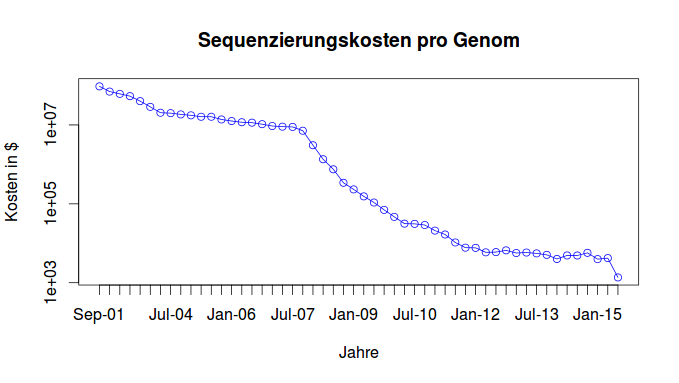
\includegraphics[width=1\linewidth]{figures/costs.png}}
\caption{\label{fig:costs}\footnotesize Trend der Genomesequenzierungskosten (NHGRI). Der starke Einbruch der Kosten im Jahr 2007 wird mit dem Übergang von Sanger-bastierten Sequenzierung zu 'second generation' oder 'next-generation'-Technologien erklärt \cite{sequencingCosts}.}
\end{figure}

% Neben den Kosten zeigt die Grafik das sogenannte Mooresche Gesetz. Es beschreibt den langzeit Trend in der Computer Hardware Industrie.
Die typische Form der Speicherung einer solchen DNS-Sequenz, ist das textbasierte FASTA Format. Es speichert die Sequenz, sowie einen vorangestellten Namen oder Kommentar, zeichenweise im ASCII-Code ab. Ein ASCII-kodierter Buchstabe verbraucht ein Byte. Vernachlässigt man den geringen Einfluss des Sequenznamen, ist die Größe der gespeicherten Datei damit proportional zur Länge der Sequenz. Am Beispiel eines Humangenoms mit einer Gesamtlänge von ca. 3 Milliarden Basenpaaren (haploid) ergibt sich eine Dateigröße von rund ~3GB (Gigabyte). Untersucht man in einer Studie 1,000 Genome von Patienten, führen dadurch allein die reinen Sequenzdaten ohne Qualitätsinformation zu einem Speicheraufkommen von ~3TB (Terrabyte). Obwohl bis jetzt erst wenige Studien eine solche Vielzahl an Sequenzierungen realisieren konnten, werden in Zukunft immer mehr Projekte wie das \textit{1000 Genome Preject}\cite{1000genomes} erwartet. Der Grund dafür ist, dass es mit Hilfe von Next-Generation-Sequencing (NGS) in den letzten Jahren für viele Firmen und Institutionen immer erschwinglicher geworden ist, DNS-Proben zu sequenzieren (Grafik \ref{fig:costs}).

Zwar sinken ebenfalls die Kosten für die Speicherung, allerdings ist der Fortschritt in der Sequenzierungstechnologie dem der Hardware Industrie weit voraus \cite{sequencingCosts}.  Das Resultat sind immer größere Mengen an produzierten Daten. Sie stellen nicht nur für die langfristige und sichere Speicherung eine Herausforderung dar, sondern auch für deren Transfer und Analyse. Um diesen Problemen entgegenzuwirken, ist ein vielversprechender Lösungsansatz die Kompression der Daten. Da Sequenzdaten generell textbasiert gespeichert werden, finden die Grundlagen der Kompression von Texten Anwendung. \\

Ziel der Kompression ist es, eine Datei in einer Art und weise zu Verändern, bzw. zu Kodieren, sodass die dabei entstehende Version weniger Speicherplatz (in Byte gemessen) als vorher benötigt. Es wird grundsätzlich zwischen verlustfreier und verlustreicher Kompression unterschieden. Da bei DNS-Sequenzen schon kleinste Unterschiede von großer Bedeutung sein können (z.B. ein Single Nucleid Polymorphism (SNP)), wird eine verlustreiche Kompression vermieden und soll in dieser Arbeit nicht weiter thematisiert werden. Weiterhin kategorisiert man Algorithmen nach bit-manipulierender, statistischer und Wörterbuch-basierter Kompression.

Die Idee der Bit-Manipulation ist es zwei oder mehr Zeichen als mit Hilfe von Bit-Kodierung in einem einzigen Byte zu speichern. Durch verschiedene Kombinationen und limitierte Alphabete können so Kompressionsraten von 1:4 erreicht werden \cite{rani14new}. Statistische Methoden entwickeln Modelle, welche das nächste Zeichen voraussagen oder die abgeleiteten Häufigkeiten für eine sinnvolle Kodierung verwenden. Wörterbuch-basierte Methoden hingegen benutzen Substitution, um wiederholt auftretende Teilsequenzen durch einen Zeiger auf einen entsprechenden Wörterbucheintrag zu ersetzen. 

Einer der am häufigsten als Basis benutzte Wörterbuch-basierten Algorithmen ist der Lempel-Ziv-Welch-Algorithmus (LZW) \cite{Ziv77auniversal}. Er komprimiert verlustfrei jedes Format, da das dynamisches Wörterbuch erst bei Start des Verfahrens aufgebaut wird. Eine weitere, sehr wichtige Methode, ist die Huffman-Kodierung \cite{huffman}. Sie weist einer festen Anzahl von Symbolen eine Bit-Codierung (Codewort) mit variabler Länge zu. Dabei bekommen häufig auftretende Symbole die kürzesten Codewörter, um so die Eingabe mit optimaler (kleinster) Länge zu kodieren. Oft werden beide Algorithmen kombiniert (\cite{software:gzip}).

Im Zuge der immer größeren Nachfrage nach speicherplatzeffizienten Formaten für DNS, wurde noch eine weitere Art der Kompression entwickelt.

Die \emph{referentielle Kompression} geht auf die spezifischen Eigenschaften von von DNS ein. Ähnlich der Wörterbuch-basierten Variante, werden bei der referentiellen Kompression ebenfalls Zeiger verwendet. Sie verweisen allerdings auf Teile einer Referenzsequenz anstatt eines Wörterbucheintrags. Man macht sich hierbei die Tatsache zu Nutze, dass, besonders innerhalb einer Spezies, die Ähnlichkeit zwischen Sequenzen sehr hoch ist. Beispielweise unterscheiden sich zwei zufällige Humangenome im Durchschnitt um nur ca. 0,1$\%$ \cite{Venter16022001}. Folglich kann man 99,9$\%$ der Sequenz als Zeiger auf eine Referenz kodieren und sollte somit eine sehr hohe Kompression erreichen können. Der Nachteil dieses Verfahrens ist die starke Abhängigkeit von der verwendeten Referenz. Vergleicht man ein Humangenom mit z.B. einem Mausgenom würde man nur eine geringe Kompression erreichen können. \cite{wandelt14trends} schätzt die Länge von gleichen Teilsequenzen zwischen Maus und Mensch auf nur ca. 20-25 Basen, wodurch eine Kodierung ähnlich der Grafik~\ref{fig:refKomp}, mehr Speicherplatz als vorher verbrauchen würde. Folglich ist die referentielle Kompression weitestgehend für sogenannte Resequenzierungs-Projekte (\textit{resequencing}) geeignet, welche sich auf die Sequenzierung von Genomen innerhalb einer Spezies konzentrieren. \\

\begin{figure}
\centering{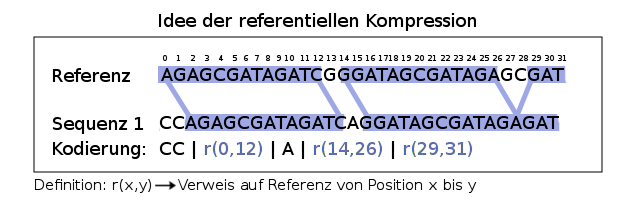
\includegraphics[width=0.8\linewidth]{figures/referentielle_kompression.png}}
\caption{\label{fig:refKomp}\footnotesize Idee der referentiellen Kompression. }
\end{figure}

Es existieren bereits einige Algorithmen und Programme mit verschiedenen Ansätzen für die referentiellen Kompression von DNS. Methoden die auf die Kompression von Rohdaten in Form von \textit{reads} abzielen (\cite{deorowicz11fastq}) werden vernachlässigt, da sie trotz ähnlicher Problemstellung nur sehr gering auf das Ziel dieser Arbeit übertragbar sind. Der Fokus liegt auf Algorithmen für die Kompression von ganzen Genomen bzw. Genomsammlungen.
Erste erfolgreiche Resultate konnten 2008 von \cite{christley09email} verzeichnet werden: Das James Watson Genom wurde von ~3.1 GB auf lediglich ~4.1 MB komprimiert. Allerdings wurde hierbei das Wissen von genauen Unterschieden, namentlich SNP's und kurze Indel's, zum Referenzgenom vorausgesetzt. Das heißt, die Eingabe für den Algorithmus ist das durch \textit{Variant Calling} vorprozessierte VCF-Format (\textit{Varaint Calling Format}). Ebenfalls auf VCF-Basis erzielte \cite{deorowicz13TDC} die bisher höchste Kompressionsrate von ca. 1:15000, auf den Daten des \textit{1000 Genome Projects}.

Das Problem des Variant Calling ist jedoch äußerst schwierig, denn es erfordert ein perfektes globales Alignment zum entsprechenden Referenzgenom. Häufig kann diese nötige Voraussetzung  nicht erfüllt werden. Aus diesem Grund muss zu den Algorithmen, welche auf reinen Sequenzdaten (FASTA-Format oder ähnliches) arbeiten können, unterschieden werden. Eine Übersicht dieser Algorithmen bis 2013 ist in Tabelle \ref{tab:software} dargstellt ~\cite{deorowicz13info}.

\begin{table}[h]
\caption{\label{tab:software}Gekürzte Originaltabelle~\cite{deorowicz13info} zu bestehenden Kompressionsalgorithmen.}
\begin{tightcenter}
\begin{tabular}{|l c c  l|}
	\toprule
	\bf Name & \bf Compression Speed      & \bf Compression Ratio & \bf Methods \\
	\midrule
	gzip & low & very low & LZ, Huf \\ 
	bzip2 & low & very low & BWT, Huf \\ 
	7z & low & high & LZ, AC \\ 
	GReEn & high & high & M.Models, AC \\ 
	GRS & moderate & high & LCS, Huf \\ 
	RLZ & moderate & high & LZ, Gol \\
	ABRC & high & very high & LZ, Huf \\ 
	GDC & high & very high & LZ, Huf \\
	\bottomrule 
\end{tabular}
\end{tightcenter}
\begin{tablenotes}
	\footnotesize
	\item \emph{Abkürzungen:} AC-arithmetic coding, Golomb (a statistical coding method), Huf-Huffman, LCS-longest common subsequence, LZ-an algorithm of the Lempel-Ziv familiy, M.models-markov models.
\end{tablenotes}
\end{table}

Die Programme gzip, bzip2 und 7z (Referenzen notwendig?), sind allgmeine, textbasierte Kompressoren, deren Kompression, unter Ausnahme von 7z, sehr gering eingeschätzt wird. Tatsächlich erzielt das sehr verbreitete Programm gzip lediglich eine Rate von ca. 1:4 (???nachgucken referenz).
Dagegen erzielen die speziell für genomische DNS entworfenen Programme deutlich bessere Ergebnisse. Die zwei Algorithmen GRS~\cite{wang11GRS} und GreEn~\cite{pinho12Green} verzeichnen Kompressionsraten für einzelne Humangenome von ca. 1:200. Während GRS als Basis das Prinzip der \textit{Longest Common Subsequence} mit anschließender Huffman-Codierung benutzt, verwendet GreEn einen statistischen Ansatz mit Hilfe Markov-Modellen. Ein Ansatz mittels der Lempel-Ziv Methode LZ77 wird von \cite{Kuruppu:RLZ} vorgeschlagen (RLZ) und erreicht ähnliche Kompressionraten von 1:250. Ein weiterer Kompressionsalgorithmus (ABRC) wurde von Wandelt und Leser angeboten, der einen komprimierten Suffixbaum für die Suche von Gemeinsamkeiten blockweise aufbaut \cite{wandelt:ABRC}. Durch anschließende Lempel-Ziv Transformation und Huffman-Kodierung erreicht das Programm ABRC Kompressionsraten von 1:400 auf Daten des \textit{1000 Genome Projects}. Eine noch höhere Kopressionsrate erreichte der Algorithmus GDC (Rate ca. 1:600) bzw. GDC Ultra (Rate ca. 1:2000) \cite{deoriwicz:GDC}, gefolgt von GDC 2 (Rate ca. 1:9000) \cite{deoriwicz:GDC2}. Ähnlich dem Programm RLZ basiert der GDC/GDC-Ultra/GDC 2 Algorithmus auf LZ77,  allerdings mit einem wichtigen Unterschied zu anderen Methoden. Alle vorherigen Methoden komprimieren auch bei einer Sammlung von Genomen jedes einzelne unabhängig. Im Gegensatz dazu, werden bei GDC mehrere Sequenzen als Referenz genutzt. Die zusätzliche Zusammenführung von Informationen zwischen den zu komprimierenden Sequenzen, stellt sich als sehr vielversprechende Idee da.\\

Über die Anstrengungen zur Reduzierung des Speicherplatzes und des Datentransfers hinaus, muss auch die zeitaufwändige Analyse solcher Datenmengen beachtet werden. Alle bisher angesprochenen Algorithmen, dienen lediglich der Kompression von Daten hinsichtlich ihrer Speicherung. Will man die Daten analysieren, müssen sie wieder dekodiert werden. Die Sequenzen bzw. Genome würden zudem einzeln und nacheinander untersucht werden. Man verwirft dabei die vorher zur Kompression benutzte Information der hohen Ähnlichkeit zwischen Sequenzen, was zur überflüssigen Analyse von redundanten Teilsequenzen führt. Es liegt folglich nahe, die referentielle Kompression auch auf die Analyse zu erweitern. Diese Problemstellung wird von \cite{loh12compressivegenomics} als \textit{compressive genomics} benannt. 

Die erste Möglichkeit, verschiedene sequentielle Algorithmen auf mehreren Sequenzen gleichzeitig laufen zu lassen, wird von \cite{Rahn15072014} vorgestellt. Durch eine unterliegende Datenstruktur, als \textit{journaled string tree} (JST) bezeichnet, werden Sequenzen als eine Menge von Varianten, basierend auf einem gemeinsamen Koordinatensystem repräsentiert. Eine einzelne Sequenz kann wiederum aus ihren zugehörigen Varianten, als referentiell komprimierter String (\textit{journaled string}), generiert werden. Durch die referentielle Kompression von Sequenzen zu Varianten, werden gemeinsame Bereiche nur einmal analysiert und die Laufzeit wird um den Faktor 115 Beschleunigt \cite{Rahn15072014}.

Diese Arbeit beschäftigt sich mit der Implementierung eines C++ Programms innerhalb der SeqAn Bibliothek \cite{doering08seqan}, welches der verlustfreien referentiellen Kompression von DNS-Sequenzen dienen soll. Sie steht in engem Zusammenhang mit dem SeqAn Projekt des JST \cite{Rahn15072014} und ist auf dessen Kompatibilität abgestimmt.

Derzeit können zur Verwendung des JST nur Dateien im VCF-Format benutzt werden. Das Hauptinteresse liegt daher nicht nur in der bestmöglichen Speicherplatzreduzierung einer Datei, sondern in der möglichst effizienten Transformation und Speicherung der Eingabedaten (FASTA-Format o.ä.) in einem für den JST weiterverwendbares Format. 

Der vorgestellte Algorithmus soll lediglich die Unterschiede zur Referenz kodieren und dabei die Idee der Zusammenführung von Informationen zwischen den zu komprimierenden Sequenzen von \cite{deoriwicz:GDC,deoriwicz:GDC2} aufgreifen. Da viele Autoren auf die Abhängigkeit der Kompression von der verwendeten Referenzsequenz hindeuten \cite{deorowicz13info,wandelt14trends,kuruppu:refseq}, ist eine Besonderheit gegenüber anderen Arbeiten, dass die verwendete Referenzsequenz variabel sein soll. Sie wird bei jeder Eingabe neu angelegt und kann fortlaufend verändert werden, mit dem Ziel, das Speicherformat weiter zu optimieren.\\

In der folgenden Sektion wird eine detaillierte Beschreibung des Algorithmus' und dessen Implementation gegeben. Anschließend werden Ergebnisse präsentiert, die bei Anwendung des Algorithmus' auf Realdaten gesammelt wurden. Nach der Diskussion der Ergebnisse, soll eine kurze Zusammenfassung und Einschätzung die Arbeit abschließen.

%%%%%%%%% METHODEN %%%%%%%%%%%%%%%%%%%%%%%%%%%%%%%%%%%%%%%%%%%%%%%%%%%%%%%%%%%%%%
\section{Methoden}
\label{sec:methods}

\subsection{Definitionen und allgemeine Notation}
\label{sec:definitions}
Ein \emph{string} \textit{s} $=$ $s_{0}$....$s_{n-1}$, $ s_{i} \in \sum$, ist eine Sequenz der Länge $|s| = n$, auf Basis des Alphabets $\sum$. Der leere \emph{string} wird mit $\epsilon$ benannt. Ein Teil\emph{string} von \textit{s}, von Position \textit{i} bis \textit{j}, wird als \textit{s}[\textit{i},\textit{j}[ = $s_{i}$....$s_{j-1}$ angegeben. Falls $i\ge j$, wird der $\epsilon$ zurückgegeben. Der Spezialfall \textit{s}[\textit{i}, \textit{i+1}[ wird zu \textit{s}[\textit{i}] abgekürzt.  \\

Ein \emph{journaled string} gleicht einem normalen \emph{string} und wird als solcher behandelt. Der Unterschied liegt nur in der Implementation. Ein \emph{journaled string} besitzt einen Zeiger auf eine Referenzsequenz, sowie eine Menge an Veränderungen bzw. Varianten. Varianten werden mittels eines Binären Baums (\textit{journal tree}) gespeichert~\cite{Rahn15072014}.\\

Ein \emph{journal entry} ist ein Eintrag im \textit{journal tree} eines \textit{journaled string} der eine Veränderung der Referenzsequenz beschreibt. Veränderungen bzw. Varianten können eine Insertion (Hinzufügen von Zeichen) oder eine Deletion (Löschen von Zeichen) beschreiben~\cite{Rahn15072014}.\\

Ein \emph{seed} ist ein Tupel ($b_{r},b_{s},e_{r},e_{s}$) und beschreibt einen gemeinsamen Teilstring von zwei Strings $r$ und $s$. Es gilt: $r$[$b_{r},e_{r}$] $=$ $s$[$b_{s},e_{s}$]. Die Länge $|seed|$ wird definiert als $b_{r}-e_{r} = b_{s}-e_{s}$ .\\

Die Menge $S(p)$ enthält alle \emph{seeds} die an Position p in der Query-Sequenz $s$ bei der Suche gegen eine Referenz $r$ gefunden wurden: $ seed=(b_{r},b_{s},e_{r},e_{s}) \in S(p)$ falls $b_{s} = p $.\\

Ein \emph{$\Delta$-Event} $e = (pos,type,cov,ins,del)$ repräsentiert eine Veränderung einer Referenzsequenz $r$ and der Position \textit{pos}. Es kann einen von vier Typen annehmen (\textit{type}): SNP, Deletion(DEL), Insertion(INS) und strukturelle Variation(SV). \textit{cov} ist die \emph{coverage} des Events (siehe Definition von \emph{coverage}). \textit{ins} bezeichnet einen String der an Stelle \textit{pos} eingefügt wird und \textit{del} die Länge des Teilstrings $r[pos,pos+del]$ der gelöscht wird.\\

Die \emph{coverage} eines $\Delta$-Events $e$ bezeichnet die Information, auf wie vielen und welchen von $n$ Eingabesequenzen $e$ vorkommt. Hierfür wird ein binärer \emph{string} $cov$ der Länge $n$ benutzt, für den gilt: $cov[i] = 1$ falls $e$ auf Sequenz $i$ zu finden ist, $cov[i] = 0$ sonst. Die Negation von $cov$ wird wie folgt definiert: $\neg cov = \neg cov[i] ~\forall ~i= 0..n$\\

Eine \emph{dependent region} ist eine Gruppe von $\Delta$-Events, in der jedes $\Delta$-Event von mindestens einem anderen $\Delta$-Event der Gruppe abhängig ist.
Definition von Abhängigkeit: $e_{1} = (pos_{1},type_{1},seq_{1},ins_{1},del_{1})$, $e_{2} = (pos_{2},type_{2},seq_{2},ins_{2},del_{2})$, o.B.d.A gilt $pos_{1} \le pos_{2} $. Dann ist $e_{1}$ abhängig von $e_{2}$ falls: $(pos_{1}+del) > pos_{2}$.

\subsection{Konzept}

\begin{figure}
\centering{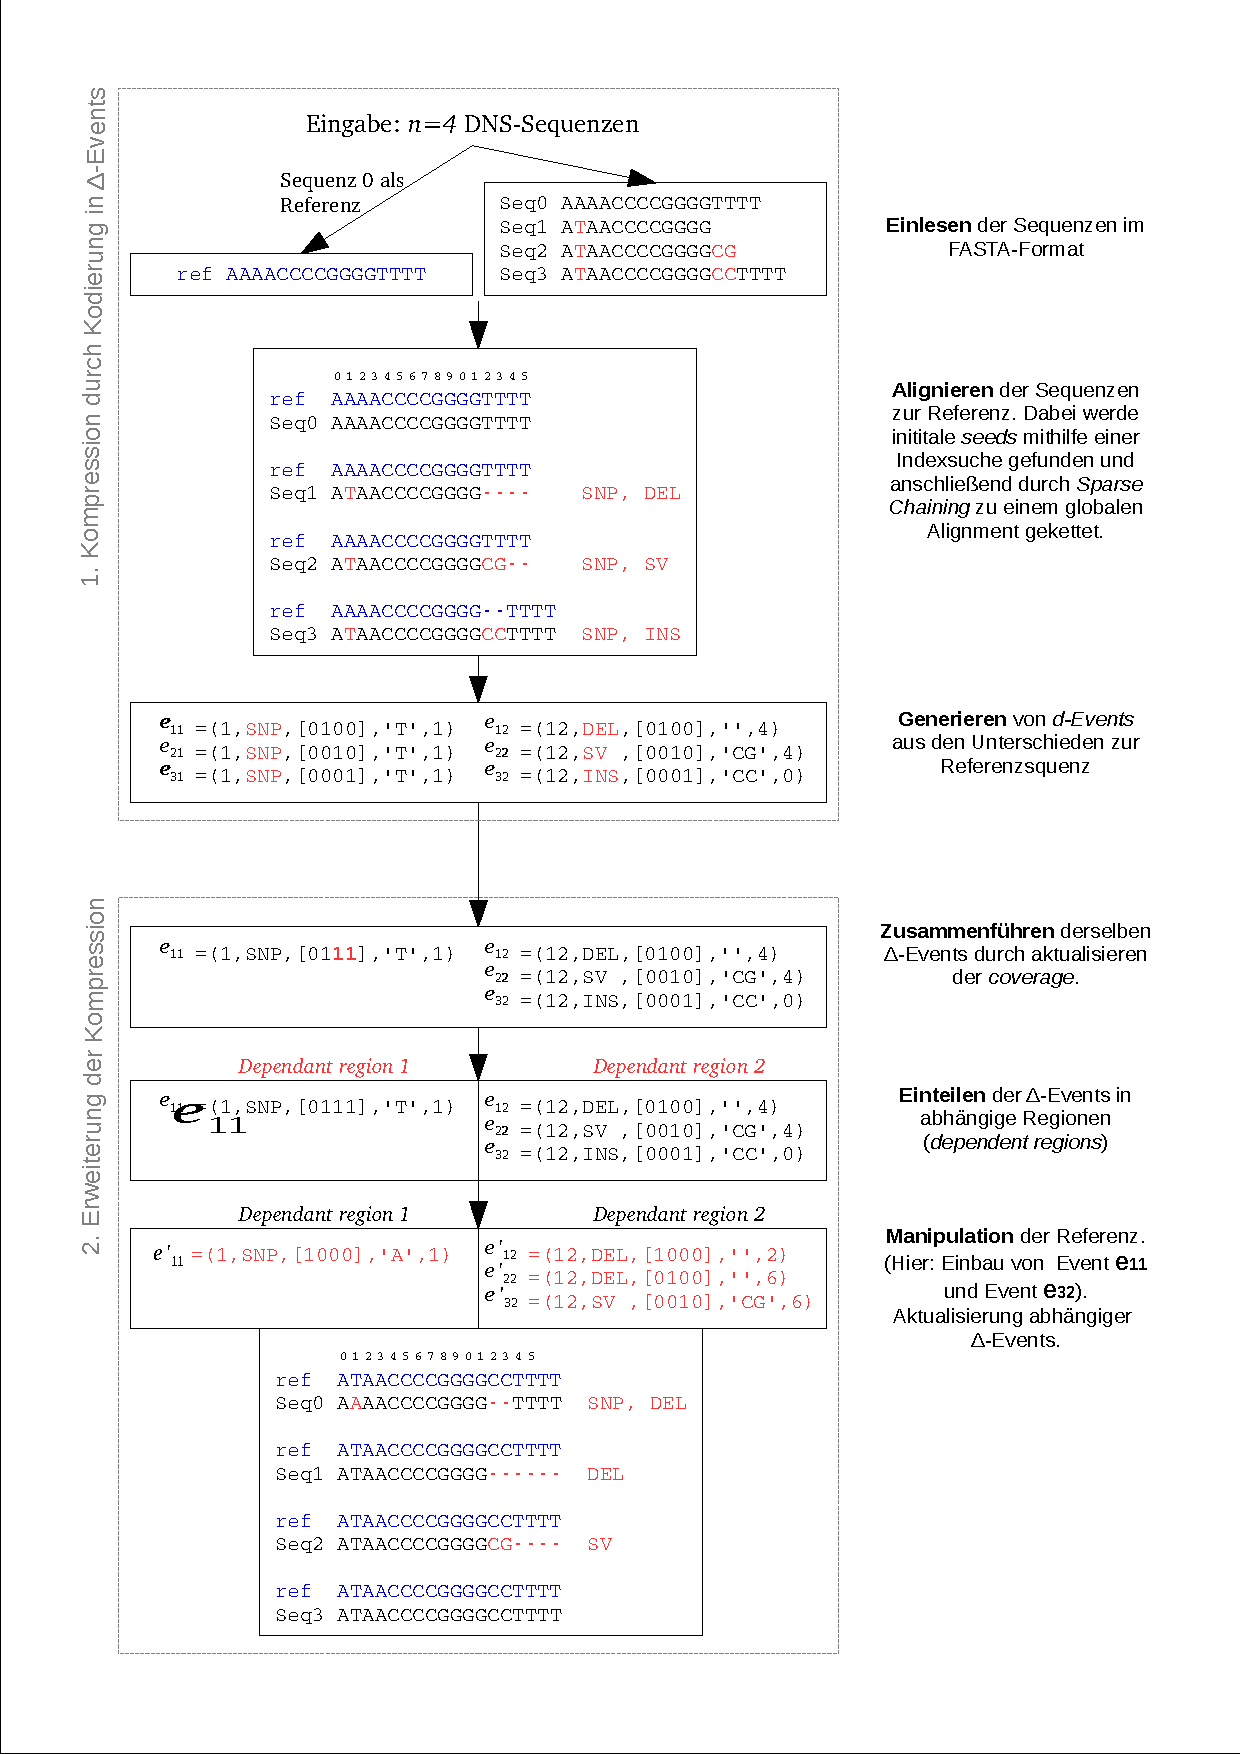
\includegraphics[width=0.9\linewidth]{figures/konzept.pdf}}
\caption{\label{fig:konzept}\footnotesize Konzept des Kompressionsalgorithmus' anhand eines Beispiels.}
\end{figure}

Der vorgestellte Algorithmus wird grundlegend in zwei Abschnitte unterteilt: Die vorläufige Kompression und deren Erweiterung. 

Zunächst werden die zu komprimierenden Eingabesequenzen im FASTA-Format eingelesen und anschließend gegen eine Referenz aligniert. Aus dem resultierenden Alignment werden nun die Unterschiede zwischen der Sequenz und ihrer Referenz als $\Delta$-Events gespeichert. Das Ergebnis ist eine referentielle Kompression der Eingabe in Form der Kodierung von Sequenzen in Unterschieden (bzw. Varianten).
%Diese Methode entspricht vom Prinzip her dem \textit{Variant Calling} zur Erstellung eines VCF-Formats (GATK~\cite{GATK:variantcalling}).

Um die Kompression zu verbessern, werden im Anschluss zusätzliche Erweiterungen vorgenommen. Hierbei werden zwei Ansätze verfolgt: (1) Die Verbesserung der Speichereffizienz und (2) die Verringerung des potentiellen Analyseaufwands.
Ersteres wird durch die Reduzierung der Anzahl an $\Delta$-Events erreicht. Der zweite Ansatz bezieht sich auf die Integration des hier vorgestellten Algorithmus' in die Arbeit von~\cite{Rahn15072014}: Die komprimierten Daten könnten weiterführend in einen JST überführt werden. Mit Hilfe des JST's können Sequenzen in Form von \textit{journal strings} effizient untersucht werden. Die Schnelligkeit des Algorithmus' hängt dabei von der Anzahl an \textit{journal entries} ab. Ziel ist es daher, durch Manipulation der Referenzsequenz, die Anzahl an potentiellen \textit{journal entries} zu verringern.

Zur Visualisierung des Algorithmus' ist ein Beispiel mit Zwischenergebnissen in Grafik~\ref{fig:konzept} dargelegt.

\subsection{Implementierung der Kompression}
\label{sec:varcall}

\subsubsection{Indexsuche}
Die Suche nach Gemeinsamkeiten zwischen einer Sequenz und ihrer Referenz ist eines der Schlüsselprobleme bei der referentiellen Kompression. In dem hier vorgestellten Algorithmus wird dazu zunächst ein q-Gram-Index über der Referenz aufgebaut. Die Wahl des Parameters q wird dem Benutzer überlassen. Allerdings wird empfohlen, das q bei genomischer DNS über 15 liegen sollte, damit zufällige q-mere vermieden werden \cite{wandelt14trends}. Da bei großen Werten für q, auf einem Alphabet $\sum$, die Anzahl an möglichen q-meren exponentiell steigt ($|\sum|^{q}$), wird ab einem Wert von 
\begin{equation}
q>log_{|\sum|}(RAM~Speicher~in~Byte)
\end{equation}
das \textit{OpenAdressing()} (SeqAn \cite{doering08seqan}) verwendet. Beim \textit{OprenAdressing()} werden nur solche q-mere gespeichert, die auch tatsächlich in der indizierten Sequenz zu finden sind.

Wird jede der $m$ Eingabesequenzen, mit einer jeweiligen Durchschnittslänge $n$, sequentiell nach gemeinsamen q-meren durchsucht, ergibt sich trotz Zugriff auf den q-Gram-Index in $O(1)$ eine Laufzeit von $O(n*m)$. Aus diesem Grund wird die Suche um einige Faktoren erweitert, die auf die spezifischen Eigenschaften von DNS eingehen.

\subsubsection{Verbesserung der Suche}
Die Indexsuche wird um folgende vier Punkte erweitert:

(1) \emph{Ignorieren von Repeats}. Genomische DNS enthält meist sehr viele repititive Abschnitte. Umfasst ein q-gram einen Repeat würde er die Suche enorm verlangsamen, denn pro q-gram in der durchsuchten Sequenz würden viele tausende in der Referenz gefunden werden. Solche q-gramme werden als Treffer ignoriert, indem jeder gefundene seed mittels seines Vorgängers auf einen Repeat getestet wird (siehe formale Definition in Sektion~\ref{sec:definitions}). Ähnlich verhält es sich auch, falls das DNS-Alphabet um den Buchstaben 'N' erweitert ist und ein q-gram ausschließlich aus 'N' besteht. Sie werden ebenfalls ignoriert.

\begin{figure}[b]
\centering{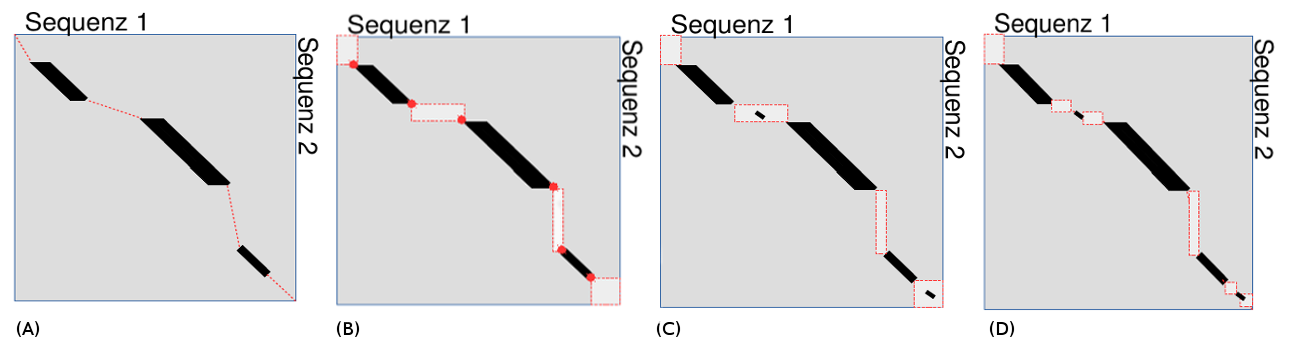
\includegraphics[width=0.9\linewidth]{figures/iterativer_schritt.png}}
\caption{\label{fig:iterativ}\footnotesize Iterative Schritte in der Indexsuche. In (A) sind in der initialen Suche drei große \textit{seeds} gefunden und für die globale Kette selektiert worden. Wie in (B) dargestellt, ergeben sich dadurch Bereiche zwischen den \textit{seeds}; Jeweils von der rechten unteren Ecke des vorhergehenden \textit{seeds} zu linken oberen Ecke des darauffolgenden. In (C) sind dadurch kleinere \textit{seeds} gefunden worden, die zu neuen Bereichen wie in (D) führen.}
\end{figure}

(2) \emph{Iterativer Schritt}(Grafik~\ref{fig:iterativ}). Die Schnelligkeit kann auf kostet der Sensitivität erhöht werden, wenn der Benutzer einen relativ hohen Wert für $q$ wählt. Um dennoch eine ausreichende Genauigkeit zu gewährleisten, können im Programmaufruf ein oder mehrere iterative Schritte mit niedrigeren Werten für $q$ spezifiziert werden. Der Algorithmus durchläuft dann eine initiale Suche mit dem ersten $q$-Wert, speichert die resultierende globale Kette und starten dann in den Bereichen zwischen den ausgewählten \textit{seeds} der Kette einen erneute Suche mit dem nächsten Wert für $q$. Diese Methode ist der des LAGAN Algorithmus für globale Alignments nachempfunden \cite{brudno03lagan}.

(3) \emph{Initiale Suche mit dynamischen Offset}. Diese Erweiterung basiert auf der Erwartung, dass bei sehr ähnlichen Sequenzen lange gleiche Abschnitte zwischen einer Sequenz und ihrer Referenz existieren. Anstatt eine sequentielle Suche (Offset=1 oder q) durchzuführen, wird in jedem Schritt der Suche ein neuer Offset bestimmt.  Hierfür wird an einer Position $p$ in der Sequenz jeder gefundene $seed_{i}(p)$ (jedes initiale q-gram) zunächst erweitert. Die Erweiterung, bzw. Verlängerung des \textit{seeds}, erfolgt solange in beide Richtungen, bis ein \textit{mismatch} (Unterschied) auftritt. Anschließend wird jedem Seed ein Score 
\begin{equation}
Score(seed)=|seed_{i}(p)|+diagonal(seed_{i}(p))
\end{equation}
zugewiesen, wobei $diagonal(seed_{i}(p))$ die Abweichung zur Hauptdiagonalen angibt. Die Länge des \textit{seeds} mit dem besten 
Score wird als neuer Offset gesetzt und die Suche auf der Sequenz wird an Position $p+offset$ fortgeführt. Etwaige Verluste an Sensitivität können durch iterative Schritte wieder ausgeglichen werden.

(4) \emph{Parallelisierung der initialen Suche}. Um die Suche abermals zu beschleunigen wird die initiale Suche parallelisiert. In Anlehnung an \cite{rani14new}, wird die zu untersuchende Sequenz in Blöcke aufgeteilt. Jeder Block wird einzeln nach Gemeinsamkeiten untersucht aber im Gegensatz zu \cite{rani14new}, werden die Blöcke vor der weiteren Analyse (und Kodierung) wieder zusammengeführt. Somit entsteht kein Informationsverlust und die Ergebnisse entsprechen denen ohne Parallelisierung.

\subsubsection{Reduktion zu einer globalen Kette}
Für die Reduktion einer Menge von \textit{seeds} wird der \textit{Sparse Chaining} Algorithmus von \cite{gusfield97algorithms} verwendet. Er konstruiert in $O(r*log(r))$ eine optimale globale Kette von \textit{seeds}, denen ein bestimmtes Gewicht (Score) zugewiesen wurde. Der Algorithmus ist bereits in der SeqAn-Bibliothek \cite{doering08seqan} enthalten und benutzt dort als Gewichtung die Länge des \textit{seeds}. Die Gewichtung ist geeignet, da längere Gemeinsamkeiten später eine geringere Anzahl an $\Delta$-Events bedeuten und somit zu bevorzugen sind.

Um die Laufzeit des Programmes zu verbessern, ist dem Benutzer möglich für den initialen Suchlauf (und nur für diesen) eine Mindestlänge der \textit{seeds} zu spezifizieren. Liegt ein gefundener \textit{seed} bei der Suche unterhalb dieser Länge wird er wieder verworfen. Mit dieser Einschränkung lässt sich die Anzahl an \textit{seeds} kontrollieren, um den \textit{Chaining}-Algorithmus zu entlasten. Auch hier wird ein drohender Verlust an Sensitivität, durch ausscheiden einiger mitunter wichtigen \textit{seeds}, mit Hilfe des iterativen Schritts ausgeglichen.

\subsubsection{Generierung von $\Delta$-Events}

\begin{figure}[t]
\centering{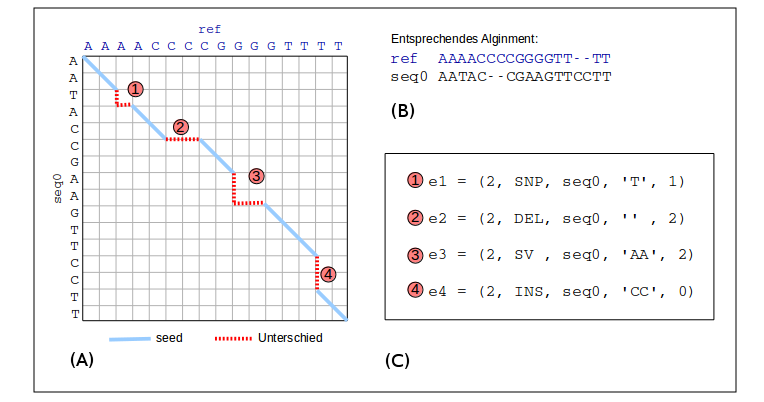
\includegraphics[width=0.9\linewidth]{figures/delta_events.png}}
\caption{\label{fig:deltaevent}\footnotesize \emph{Generierung von $\Delta$-Events}. Abbildung (A) visualisiert das Ergebnis der Indexsuche. Die Bereiche zwischen den \textit{seeds} bilden die Vorlage für die $\Delta$-Events. (B) zeigt die entsprechende Alignment-Repräsentation und (C) die generierten $\Delta$-Events.  }
\end{figure}

Steht die globale Kette fest, repräsentiert sie ein globales Alignment zwischen der untersuchten Sequenz und der Referenz. Jeder \textit{seed} beschreibt dabei eine gemeinsame Teilsequenz, wohingegen die Bereiche dazwischen Unterschiede bzw. Varianten darstellen. Jeder dieser Zwischenbereiche wird zu einem einzelnen $\Delta$-Event, indem die zwei angrenzenden \textit{seeds} mittels Manhattan-Distanz verbunden werden. Die Position eines $\Delta$-Events wird dabei als absolute Position in der Referenz gespeichert (Abbildung~\ref{fig:deltaevent}).

\emph{Formale Definition}. Man betrachte die Analyse der i-ten Sequenz $s$ (aus insgesamt $n$ Sequenzen) gegen die Referenz $r$. $seed_{1} = (b^{1}_{r},b^{1}_{s},e^{1}_{r},e^{1}_{s})$ und $seed_{2}=(b^{2}_{r},b^{2}_{s},e^{2}_{r},e^{2}_{s})$ liegen hintereinander in der globalen Kette. O.B.d.A liegt $seed_{1}$ über und links von $seed_{2}$. Dann werden aus dem Bereich zwischen $seed_{1}$ und $seed_{2}$ folgende Attribute für das Event $e$ 
\begin{equation}
e = (pos,~type,~cov,~ins,~del)
\end{equation}
definiert:
\begin{equation}
pos = e^{1}_{r}
\end{equation}
\begin{equation}
type = 
\begin{cases}
SNP & falls~ |ins| = 1~ und~ del = 1, \\
DEL & falls~ |ins| = 0, \\
INS & falls~ del = 0, \\
SV  & sonst
\end{cases}
\end{equation}
\begin{equation}
\forall j=0..n ~~cov[j] = 
\begin{cases}
1 & falls~ j = i, \\
0 & sonst 
\end{cases}
\end{equation}
\begin{equation}
ins = s[e^{1}_{s},b^{2}_{s}]
\end{equation}
\begin{equation}
del = b^{2}_{r}-e^{1}_{r}
\end{equation}

\subsection{Erweiterung der Kompression}
\label{sec:evepro}

\subsubsection{Verbesserung der Speichereffizienz}
Die Idee beruht auf der Erwartung, dass auf verschiedenen Sequenzen die selben Variationen zu finden sind. Beispielweise gibt es häufig auftretende \textit{Single Nucleotide Polymorphims} (SNP) innerhalb bestimmter menschlichen Population \cite{INFO:snp_variation}. Anstatt folglich alle Variationen einzeln zu speichern, können gleiche zusammengefasst werden.

Hierzu werden alle gesammelten $\Delta$-Events (aller Sequenzen) durchlaufen. Falls sich zwei Events in ihrer Position, ihres Typs und den Werten für \textit{del} und \textit{ins} exakt gleichen werden sie zusammengeführt. Es muss dabei lediglich die \textit{coverage (cov)} des einen Events um die entsprechende Sequenzinformation des anderen aktualisiert werden. Letzteres Event kann nun gelöscht werden, da es redundante Informationen trägt. Der binäre \textit{cov}-Vektor gewährleistet hierbei eine effiziente Speicherung und eine einfache Handhabung mittels logischer Operationen.

\subsubsection{Verringerung des potentiellen Analyseaufwands}
In der Analyse mittels eines \textit{journal string tree} (JST) benötigt man für jede zu untersuchende Eingabesequenz einen \textit{journal string}. Jeder \textit{journal string} muss dabei auf die selbe Referenz verweisen und durch die Varianten zu jener Referenz (\textit{journal entries}) seine entsprechende Ausgangssequenz darstellen. Beide Voraussetzungen sind beim Ergebnis des vorgestellten Algorithmus erfüllt: Die produzierten $\Delta$-Events haben die selbe Referenz und gleichen in ihrer Struktur den Varianten eines \textit{journal strings} (SNP, Deletion, Insertion und Strukturelle Variation). Es besteht folglich die Möglichkeit $\Delta$-Events in \textit{journal strings} zu überführen.
Bei der Überführung kann festgehalten werden, dass pro Deletion ein zusätzlicher \textit{journal entry} generiert werden würde und bei allen anderen Eventtypen zwei zusätzliche \textit{journal entries} (siehe Zusatzmaterial für detaillierte Beschreibung).
Wie bereits erwähnt, hängt die Effizienz der Analyse von der Gesamtanzahl an \textit{journal entries} ab und das Ziel dieser Erweiterung ist es daher die Anzahl an potentiellen \textit{journal entries} nach einer Überführung zu minimieren. Die Umsetzung erfolgt durch eine Manipulation der Referenzsequenz.\\

Zur Verdeutlichung soll folgendes Beispiel dienen: Angenommen die ersten acht von zehn Sequenzen unterscheiden sich zur Referenz $r$ durch den selben SNP, $A\rightarrow C$, an Position 16. Nach Zusammenführung der einzelnen SNP-Events bliebe das $\Delta$-Event $e = (16,~SNP,~cov=1111111100,~'C',~1)$. Pro Sequenz würden zwei \textit{journal entries} für den jeweiligen \textit{journal string} benötigt werden: $8*2 = 16$ \textit{journal entries}. Man kann nun eine Veränderung der Referenz an Position 16 von A auf C in Erwägung ziehen. Durch diese Veränderung würde aus $e$ das Event $\tilde{e} = (16,~SNP,~cov=0000000011,~'A',~1)$ entstehen, welches zwar den selben Speicherplatz benötigt, bei einer Überführung aber nur $2*2=4$ \textit{journal entries} erfordern würde.
\\

Um diese Idee generisch auf alle $\Delta$-Events anwenden zu können, müssen diese zuerst in Gruppen, sogenannte \emph{dependent regions} (siehe Defintionen), eingeteilt werden. Diese Einteilung ist notwendig, da bei einer Änderung der Referenz bezüglich $e$, die von $e$ abhängigen Events gesondert betrachtet und geändert werden müssen. Eine fehlerfreie Kodierung ist sonst nicht mehr gewährleistet.

Die Zuteilung verläuft wie folgt: Gegeben sei $\Delta$-Event $e_{j}$ in einer aufsteigend sortierten Liste von $\Delta$-Events, sowie $e_{j-i} \in G$. Ist $e_{j}$ abhängig von $e_{j-1}$, wird $e_{j}$ zu $G$ hinzugefügt. Andernfalls ist $G$ vollständig und es wird eine neue Gruppe mit $e_{j}$ als erstem Element initiiert.

Alle weiteren Schritte werden gruppenweise durchgeführt.\\

Zunächst wird für alle $\Delta$-Events einer Gruppe ein Score berechnet. Der Score eines Events $e$ wird definiert als die Anzahl an \textit{journal entries}, welche durch den Einbau von e in die Referenz hinzukommen oder wegfallen würden. Ein negativer Score drückt daher aus, dass eine Änderung der Referenz durch den Einbau von $e$ von Vorteil wäre, da die Anzahl an \textit{journal entries} verringert werden würde.

Das $\Delta$-Event mit dem besten (am meisten negativen) Score wird nun in die Referenz eingebaut. Der Einbau in die Referenz bedeutet, dass die Änderungen, die $e$ beschreibt, in die Referenzsequenz $r$ übernommen werden. Es wird die Teilsequenz $r[pos_{e},~pos_{e}+del_{e}]$ aus $r$ gelöscht und die Teilsequenz $ins_{e}$ an Position $pos_{e}$ eingefügt. Aufgrund der Änderung der Referenz sind nun die übrigen Kodierungen der Sequenzen falsch und müssen aktualisiert werden. Bei einer Aktualisierung wird zwischen Sequenzen, welche abhängige Events zu $e$ besitzen und denen die unabhängig sind, unterschieden. 

Für die unabhängigen oder nur indirekt abhängigen Sequenzen muss lediglich ein neues Event $\tilde{e}$ erstellt werden. $\tilde{e}$ kann als gegenteiliges Event zu $e$ gesehen werden und wird definiert als:
\begin{equation}
\tilde{e} = (pos_{e},~\neg type_{e},~\neg cov_{e},~r[pos_{e},~pos_{e}+del_{e}],~|ins_{e}|)
\end{equation}
wobei
\begin{equation}
\neg type_{e} =
\begin{cases}
DEL & falls~ type_{e} = INS, \\
INS & falls~ type_{e} = DEL, \\
type_{e} & sonst
\end{cases}
\end{equation}
\\

Für Sequenzen mit von $e$ abhängigen Events muss jedes Event einzeln aktualisiert werden. Gegeben sind das in die Referenz einzubauende Event $e$ und ein von $e$ abhängiges Event $e'$; Dann wird $e'$ wie folgt aktualisiert:

\noindent Falls $pos_{e} \le pos_{e'}$
\begin{equation}
k_{e} = (pos_{e'},~*type,~cov_{e'},.........)
\end{equation}
Falls $pos_{e} \ge pos_{e'}$
\begin{equation}
k_{e} = (pos_{e'},~*type,~cov_{e'},.........)
\end{equation}
* wobei jeweils $type$ anschließend wie Gleichung (6) ermittelt wird.\\

\noindent Nach erfolgreicher Manipulation der Referenz werden alle Schritte für die aktualisierten Events der Gruppe wiederholt. Falls kein $\Delta$-Event mehr für vorteilhaft befunden wird, wird mit der nächsten Gruppe fortgefahren.

\pagebreak
%%%%%%%%% RESULTS %%%%%%%%%%%%%%%%%%%%%%%%%%%%%%%%%%%%%%%%%%%%%%%%%%%%%%%%%
\section{Ergebnisse}
Die Auswertung wurde auf einem internen Server mit Linux 3.13.0 System mit .... two Intel\textregistered Core\texttrademark i5-3317U CPU's at 1.70GHz (a total of 2 physical and 2 virtual cores) and 5.8GB of RAM. 

Das Programm wurde auf Realdaten getestet. Der erste Datensatz besteht aus bis zu 200 Versionen des menschlichen Chromosoms 22 erhalten vom \textit{1000 Genome Project}~\cite{1000genomes}. Alle Varianten der 1000 Individuen sind einer VCF-Datei gespeichert und mussten für die Analyse zurück in einzelne FASTA-Dateien überführt werden. Hierfür wurde vcf-subset aus dem Paket vcf-tools benutzt, um den VCF-Datensatz auf einzelne Individuen zu reduzieren. Anschließend wurde mittels GATK -Genome..bla.bla aus dem VCF-Format und der im Projekt angegebenen Referenz die entsprechende FASTA-Datei generiert. Der zweite Datensatz besteht aus 20 E.Coli Genomen bereitgestellt durch EcoliWiki.net \cite{DATA:ecoli}.

Der Kompressionsalgorithmus besitzt folgende Parametereinstellungen:
\begin{table}[h!]
\centering{
\begin{tabular}{lll}
\hline
\\
Kürzel & Parameter & Beschreibung \\
\hline
\\
-$h$   & - -$help$         & \small Displays this help message.\\
-$v$   & - -$version$      &  \small Display version information.\\
-$i$   & - -$input\_file$  & \small Path to the input file. Valid filetype: FASTA.\\
-$q$   & - -$q\_gram$       & \small Size of the q-gram(-index) when finding seeds.\\ 
       &                   & \small Define multiple times for iterative search.\\
-$t$   & - -$threads$      & \small The number of threads that can be used.\\
-$mss$ & - -$maximum\_seed\_size$ & \small The threshold in the first seeding step for the \\
       &                          & \small maximum seed size.\\
-$ev$  & - -$evaluation$  & \small If set, this will trigger an evaluation of the\\
       &                  & \small performed algorithm.\\
\\
\hline
\end{tabular}
}
\caption{\label{tab:parameter}\emph{Parameter des SeqAn Tools für referentielle Kompression}.}
\end{table}

\subsection{Evaluation der Indexsuche}
Das durch die Indexsuche produzierte Alignment ist kein optimales globales Alignment aber es sollte sich diesem idealerweise annähern. 

Abbildung~\ref{fig:seeds} zeigt den Vergleich von im Voraus bekannten VCF-Einträgen zu den bei der Indexsuche gefundenen \textit{seeds}. Es ist eine starke Korrelation der jeweiligen Graphen erkennbar. Die Ergebnisse in Abbildung~\ref{fig:seeds} wurden mit dem Parametern $q=20$ (initial) und $q=15$ (iterativer Schritt) durchgeführt. Das bedeutet, dass Varianten die weniger als 15 Basen von einander entfernt liegen, nicht separat erkannt werden und folglich als eine einzelne große Variante gespeichert werden. Im Durchschnitt der sechzehn untersuchten Individuen, haben $3792$ Varianten einen geringeren Abstand als 15 Basen zu Ihrem Vorgänger. Diese Zahl liegt nahe der absoluten Differenzen zwischen der Anzahl an VCF-Einträgen und der Anzahl von \textit{seeds}.

\begin{figure}[t]
\centering{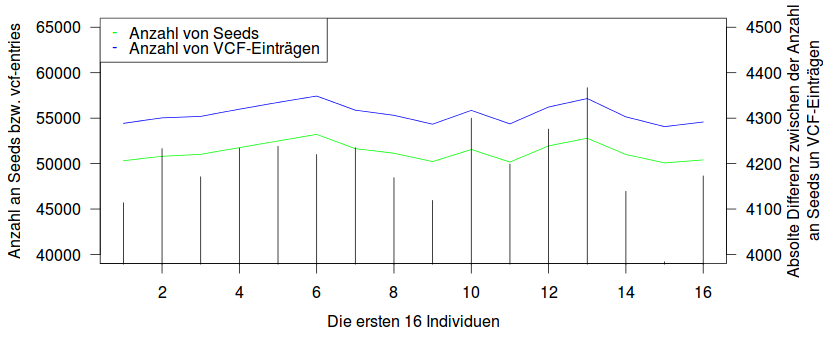
\includegraphics[width=0.9\linewidth]{figures/seedsVSvcf.png}}
\caption{\label{fig:seeds}\footnotesize \emph{Vergleich der Anzahl von Seeds gegen die zugrunde liegenden VCF-Einträge}. Der blaue Graph zeigt die Anzahl an Varianten der Referenzdatei des 1000 Genome Project. Der grüne Graph zeigt die entsprechende Anzahl an gefundenen Seeds als Ergebnis der Indexsuche. Die Indexsuche wurde mit dem Parameter $q=20$ und im Iterativen Schritt mit $q=15$ auf 16 Kernen durchgeführt, mit einer initialen Mindestgröße für Seeds von 100 . Die hinzugefügten Balken zeigen die absolute Differenz zwischen beiden Graphen.}
\end{figure}

\subsection{Leistung beim menschlichen Chromosoms 22}
\begin{table}[t]
\caption{\label{tab:space}\emph{Übersicht der Kompressionsergebnisse von Chromosom 22}.}
\small
\begin{tightcenter}
\begin{tabular}{lccccccc}
	\toprule
	$\#$Seq & Rohdaten & \multicolumn{3}{c}{Kompression auf Datei-Ebene} & \multicolumn{3}{c}{Kompression auf JS-Ebene}\\
              &\tiny[MB] & Vorher\tiny[MB] & Nachher\tiny[MB] & \textbf{Ratio}       & Vorher\tiny[MB] & Nachher\tiny[MB] &  \textbf{Ratio}  \\
	\midrule
	10        &  573.72  &    7.24    &    2.29     &  \textbf{250.16}     &    12.93   &     7.28    &  \textbf{78.82}  \\
	50        & 2659.97  &   36.08    &    7.02     &  \textbf{378.94}     &    64.19   &     34.83   &  \textbf{76.38}  \\
	100       & 5215.63  &   71.68    &    12.77    &  \textbf{408.56}     &   127.49   &     69.03   &  \textbf{75.55}  \\
	200       & 10431.27 &  144.08    &    24.69    &  \textbf{422.50}     &   256.47   &    139.53   &  \textbf{74.76}  \\
	\bottomrule
\end{tabular}
\end{tightcenter}
\begin{tablenotes}
	\small
	\item \emph{Anmerkung.} Die Bezeichnung \textit{Vorher} bezieht sich auf das Ergebnis vor den in Sektion \ref{sec:evepro} beschriebenen Verbesserungen: Auf Datei-Ebene vor der Zusammenführung von Events und auf Journaled String (JS)-Ebene vor der Prozessierung von Events. Das Verhältnis (Ratio) bezieht sich jeweils auf die \textit{'Nachher'}-Werte zu den entsprechenden Rohdaten.
\end{tablenotes}
\end{table}

\begin{table}[t]
\caption{\label{tab:runtime}\emph{Übersicht der Performance}.}
\small
\begin{tightcenter}
\begin{tabular}{lcccc}
	\toprule
	$\#$Chr 22 & Rohdaten & \multicolumn{2}{c}{Laufzeitanalyse} & Speicherverbrauch\\
               & \tiny[MB]     & ohne Proz.\tiny[MB/s] & mit Proz.\tiny[MB/s]            & \tiny[MB] \\
	\midrule
	10  &  573.72  & 7.39 & 2.68 & 4.72\\
	50  & 2659.97  & 8.71 & 5.31 & 9.84\\
	100 & 5215.63  & 9.12 & 6.28 & 16.49\\
	200 & 10431.27 & 8.95 & 6.86 & 30.32\\
	\bottomrule
\end{tabular}
\end{tightcenter}
\begin{tablenotes}
	\small \centering
	\item \emph{Anmerkung.} Ohne/mit Proz. = ohne/mit nachfolgender Prozessierung von Events.
\end{tablenotes}
\end{table}

\begin{figure}[h]
\centering{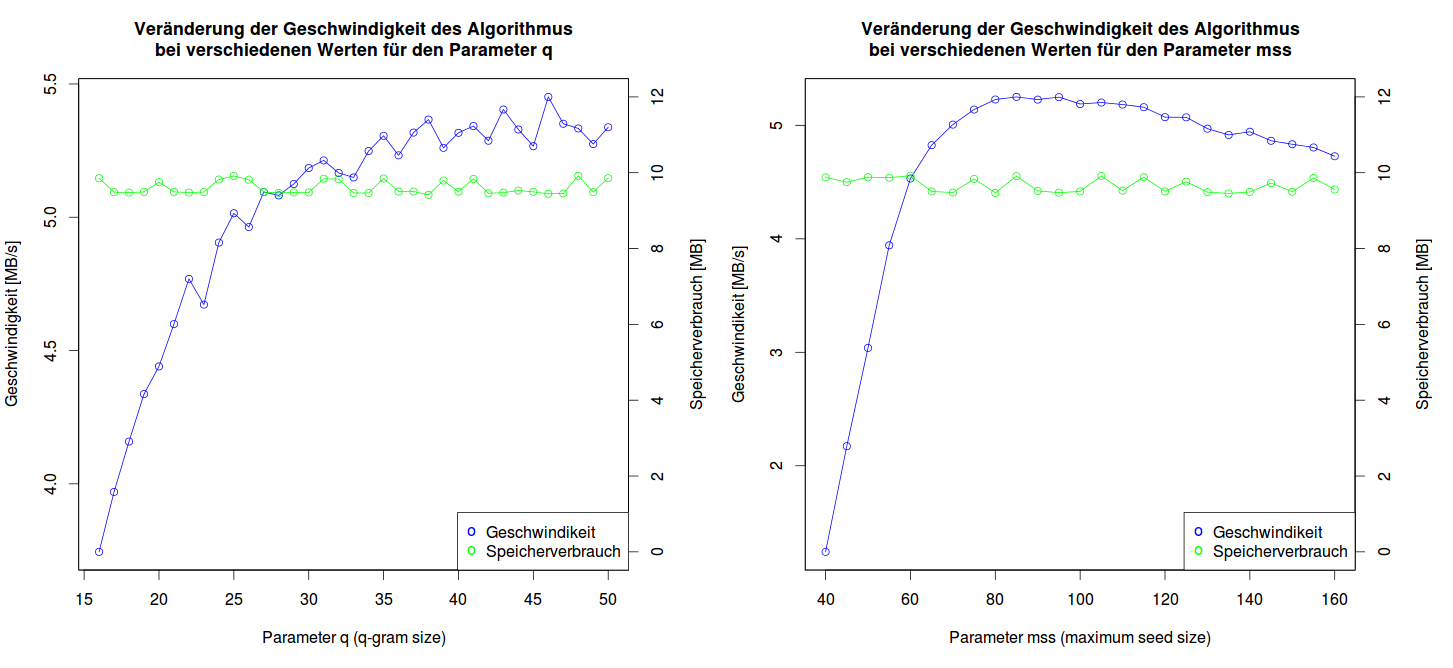
\includegraphics[width=1\linewidth]{figures/parameters.png}}
\caption{\label{fig:param}\footnotesize \emph{Einfluss der Parameter $q$ (q-gram Größe) und $mss$ (Maximale \textit{seed} Größe)}. Die Untersuchungen wurden mit einer Anzahl von 50 Chromosomen 22 durchgeführt.}
\end{figure}


Der Kompressionsalgorithmus wurde auf einer verschiedenen Anzahl an menschlichen Chromosomen 22 getestet. Für alle 4 Datensätze (Anzahl 10, 50, 100 und 200 Sequenzen) wurden folgende Parametereinstellungen gewählt:\\

\begin{lstlisting}[style=BashInputStyle]
    $ compressFASTA -i input.fa -q 35 -q 15 -mss 100 -t 16 (-ev)
\end{lstlisting}

Auf den Parameter -$ev$ wurde zur Laufzeit- und Arbeitsspeicheranalyse verzichtet.\\

\noindent Die resultierenden Ergebnisse hinsichtlich der Kompression sind in Tabelle~\ref{tab:space} aufgelistet. Es wird zwischen dem Speicheraufwand bei der Kompression auf Datei-Ebene und der Kompression auf \textit{Journaled String}-Ebene unterschieden.

\emph{Die Kompression auf Datei-Ebene} zielt auf die Reduzierung des Speicheraufwands einer gespeicherten Ergebnisdatei ab. Die generierten (vorher) und zusammengeführten (nachher) $\Delta$-Events können als solche in einer Datei gespeichert werden. Bisher wurde noch kein entsprechendes Ausgabeformat erstellt, weswegen die angegeben Werte hypothetischen Berechnungen entsprechen. Dabei werden für die Attribute $pos$, $type$ und $del$ jeweils ein \textit{unsigned integer} (4 Byte) und für den Bitvektor $cov$ eine ungefähre Größe von $\#$Sequenzen/8 Byte (8 Bit pro Byte) berechnet. Der Wert für $ins$ wird bei der Ausgabe des Programms für jede Sequenz angegeben (vorrausgesetzt -$ev$ wurde spezifiziert). Je höher die Anzahl an zu komprimierenden Sequenzen, desto bessere Kompressionsverhältnisse werden erreicht. Vergleichbare Ergebnisse liefern die Algorithmen ABRC~\cite{wandelt:ABRC} und GDC~\cite{deoriwicz:GDC} die ebenfalls auf dem Datensatz des \textit{1000 Genome Projects} arbeiten. ABRC erreicht auf 1000 Sequenzen im Durchschnitt ein Kompressionsverhältnis von 1:397~\cite{wandelt:ABRC}, während GDC bei 1092 Chromosomen 22 ein Verhältnis von 1:823 erzielt (durchschnittlich 1:627)~\cite{deoriwicz:GDC2}.

\emph{Die Kompression auf Ebene der \textit{Journaled String}} erzielte geringere Verhältnisse. Dabei ist es wichtig anzumerken, dass die Zusammenführung von Events keine Auswirkungen auf die Anzahl an Journal Entries hat, da jede Sequenz individuell und unabhängig aufgebaut werden muss. Zur Berechnung des Speicheraufwands eines Journaled Strings ...............  \\

Die Performance des Algorithmus' ist in Tabelle~\ref{tab:runtime} zu sehen. Die Laufzeit wird dabei in bedeutendem Maße von der Wahl an Parametern beeinflusst (siehe Grafik\ref{fig:param}).

Zum Vergleich mit anderen Kompressionsalgorithmen muss die Laufzeit ohne Prozessierung betrachtet werden, da andere Algorithmen keine weiterverarbeitende Datenstruktur zur Verfügung stellen. Algorithmen zur Kompression einzelner Sequenzen erreichen Geschwindigkeiten von ca. 1.2 MB/s (GRS \cite{wang11GRS}) und 8.2 MB/s (GreEn \cite{pinho12Green}). Die vorher angesprochenen Algorithmen erreichen sogar durchschnittlich 40 MB/s (ABRC~\cite{wandelt:ABRC}) und ca. 73 MB/s (GDC \cite{deoriwicz:GDC}).


\subsection{Leistung bei E.Coli Genomen}
\begin{table}[t]
\caption{\label{tab:space_ecoli}\emph{Übersicht der Kompressionsergebnisse von E.Coli Genomen}. }
\small
\begin{tightcenter}
\begin{tabular}{lccccccc}
	\toprule
	$\#$Seq & Rohdaten & \multicolumn{3}{c}{Kompression auf Datei-Ebene} & \multicolumn{3}{c}{Kompression auf JS-Ebene}\\
       & \tiny[MB]  & Vorher\tiny[MB] & Nachher\tiny[MB] & \textbf{Ratio} & Vorher\tiny[MB] & Nachher\tiny[MB] & \textbf{Ratio}\\
	\midrule
	5  & 30.70  & 12.17 & 11.18 & \textbf{2.75} & 14.20 & 13.06 & \textbf{2.35}\\
	10 & 55.87  & 24.29 & 22.18 & \textbf{2.52} & 28.16 & 26.08 & \textbf{2.14}\\
	20 & 113.54 & 49.98 & 41.23 & \textbf{2.75} & 60.93 & 52.84 & \textbf{2.15}\\
	\bottomrule
\end{tabular}
\end{tightcenter}
\begin{tablenotes}
	\small
	\item \emph{Anmerkung.} Die Bezeichnung \textit{Vorher} bezieht sich auf das Ergebnis vor den in Sektion \ref{sec:evepro} beschriebenen Verbesserungen: Auf Datei-Ebene vor der Zusammenführung von Events und auf Journaled String (JS)-Ebene vor der Prozessierung von Events. Das Verhältnis (Ratio) bezieht sich jeweils auf die \textit{'Nachher'}-Werte zu den entsprechenden Rohdaten.
\end{tablenotes}
\end{table}

\begin{table}[t]
\caption{\label{tab:runtime_ecoli}\emph{Übersicht der Performance}.}
\small
\begin{tightcenter}
\begin{tabular}{lcccc}
	\toprule
	$\#$Seq & Rohdaten & \multicolumn{2}{c}{Laufzeitanalyse} & Speicherverbrauch \\
            & \tiny[MB]& ohne Proz.\tiny[MB/s] & mit Proz.\tiny[MB/s] & \tiny[MB]\\
	\midrule
	10      &  30.70   &     0.19        &      2.26                   &    0.52 \\
	50      &  55.87   &     0.02        &      2.18                   &    0.83 \\
	100     & 113.54   &     0.01        &      2.13                   &    1.49 \\
	\bottomrule
\end{tabular}
\end{tightcenter}
\begin{tablenotes}
	\small \centering
	\item \emph{Anmerkung}. Ohne/mit Proz. = ohne/mit nachfolgender Prozessierung von Events.
\end{tablenotes}
\end{table}

\begin{table}[ht!]
\caption{\label{tab:anzahlen}\emph{Vergleich der Anzahlen von $\Delta$-Events bzw. \textit{Journal Entries}}.}
\small
\begin{tightcenter}
\begin{tabular}{lccccccc}
	\toprule
 	& E.Coli ($10~Sequenzen$) & menschl. Chr 22 ($10~Sequenzen$) \\
 	& [Anzahl/MB] & [Anzahl/MB] & \\
	\midrule
	$\Delta$-Events          & 2935.44 & 202.69\\
	\textit{Journal Entries} & 9064.45 & 948.42\\
	\bottomrule
\end{tabular}
\end{tightcenter}
\end{table}

Für die Untersuchung an Sequenzen mit einer geringen Ähnlichkeit untereinander wurden 20 E.Coli Genome untersucht \cite{DATA:ecoli}. Es wurden die selben Parameter wie bei der Auswertung der menschlichen Chromosomen benutzt. Die Ergebnisse für die Kompression und Performance sind in Tabelle~\ref{tab:space_ecoli} und Tabelle \ref{tab:runtime_ecoli} dargelegt. Die Kompressionsverhältnisse sind deutlich geringer als beim menschlichen Chromosom. Auch die Verbesserungen durch Zusammenführung oder Prozessierung von Events zeigen nur wenig Erfolge bei der Speicherverminderung. Die Laufzeit wäre ohne die Prozessierung von Events ähnlich der des menschlichen Chromosoms, ist mit dieser allerdings sehr langsam. 

Ein Vergleich der Anzahl an $\Delta$-Events bzw \textit{Journal Entries} pro MB an Eingabesequenz zeigt bei E.Coli sehr viel höhere Verhältnisse (siehe Tabelle~\ref{tab:anzahlen}).

Schlechtere Ergebnisse bei Sequenzen mit geringerer Ähnlichkeit sind bei allen bisher angesprochenen Algorithmen zu beobachten.
\pagebreak
%%%%%%%%% CONCLUSION %%%%%%%%%%%%%%%%%%%%%%%%%%%%%%%%%%%%%%%%%%%%%%%%%%%%%%%%%%%
\section{Disskusion und Fazit}
tralala
\pagebreak
%%%%%%%%% REFERENCES %%%%%%%%%%%%%%%%%%%%%%%%%%%%%%%%%%%%%%%%%%%%%%%%%%%%%%%%%%%
\bibliographystyle{apalike}  % Style
%\bibliographystyle{acm}  % Style
\bibliography{myBibliography.bib}

\end{document}
